\chapter{User Manual}
This is the user manual for the UrbanSearch Web Interface. Here we will discuss the various interfaces that are available in the UrbanSearch system. The manual is meant for new users of the system.

\section{General remarks}
The UrbanSearch Web Interface can be accessed by visiting \url{"http://citynetworks.bk.tudelft.nl/"}. Visiting this URL will open an interactive map on which intercity relations are visualised.\\
The front-end of the UrbanSearch system consists of several interfaces listed below. In the coming sections we will dive deeper into the functionalities offerd by the different interfaces.

\begin{description}[align=left]
\item [Map] some detail
\item [Classification] some detail
\item [Classifier] some detail
\end{description}. 


\section{The Menu}
The menu on the left of the screen displays three different sections. The first section displays an option to export the data. The second section can be used to determine what cities should be displayed on the map. The last section displays the different relation types. The thresholds cities should have for each type can be adjusted here. This section also includes an option to select other weighting models that can be used.


\subsection{Exporting Data}
The first section on the menu is an export option. Here a button is displayed which can be used to export all relations between cities in an excel file (CSV). Above this button is a field in which a probably threshold can be set for the export. 

\begin{figure}[H]
    \centering
    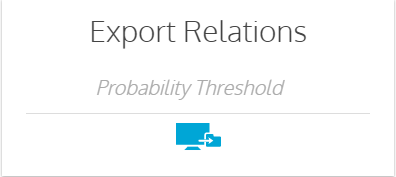
\includegraphics{export}
    \caption{Export}
    \label{fig:infoflow}
\end{figure}



\subsection{Selecting Cities}
The second section of the menu displays options for selecting which cities should be displayed on the map. A slider can be used to select a minimum and maximum population size for displayed cities. Underneath is a dropdown menu in which cities can be removed and added to the map manually. 

\begin{figure}[H]
    \centering
    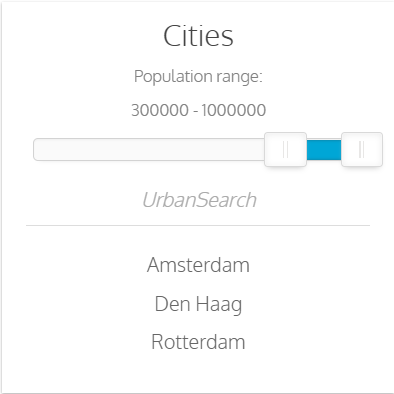
\includegraphics[scale=.74]{cities}
    \caption{Cities options}
    \label{fig:infoflow}
\end{figure}


\subsection{Selecting Relations}
In the relations section of the menu a dropdown menu is displayed which is used to select how the weights of the relations should be calculated. The standard way is to just select the occurrences of documents per relation type. However it is also possible to use a gravity model, which takes the population and the distance between cities into account. \todo{can we do this?} Beneath that are sliders for the different relationship types. Here you can change the minimum occurrences a relation type should have per two cities before the relation is taken into account. There is also an option to turn off the relation types entirely.

\begin{figure}[H]
    \centering
    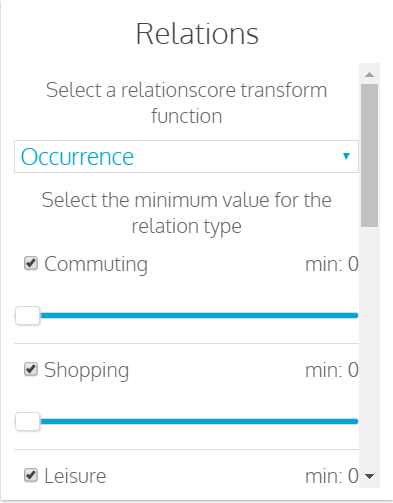
\includegraphics[scale=.74]{relations}
    \caption{Relations options}
    \label{fig:infoflow}
\end{figure}


\section{The Map}
After a few seconds needed to load the relations, a map should be displayed. This map first only contains some cities. The scroll wheel of the mouse or the plus and minus buttons in the lower right corner of the map for zooming. When hovering over a city with the mouse the population of that city will be displayed. To show the relations of a city, that city can be clicked on. The cities showing relations will have a slightly darker color than cities that have not been clicked on. You can also click on a relation. This will open up an extra window in the menu containing information about that relation.

\begin{figure}[H]
    \centering
    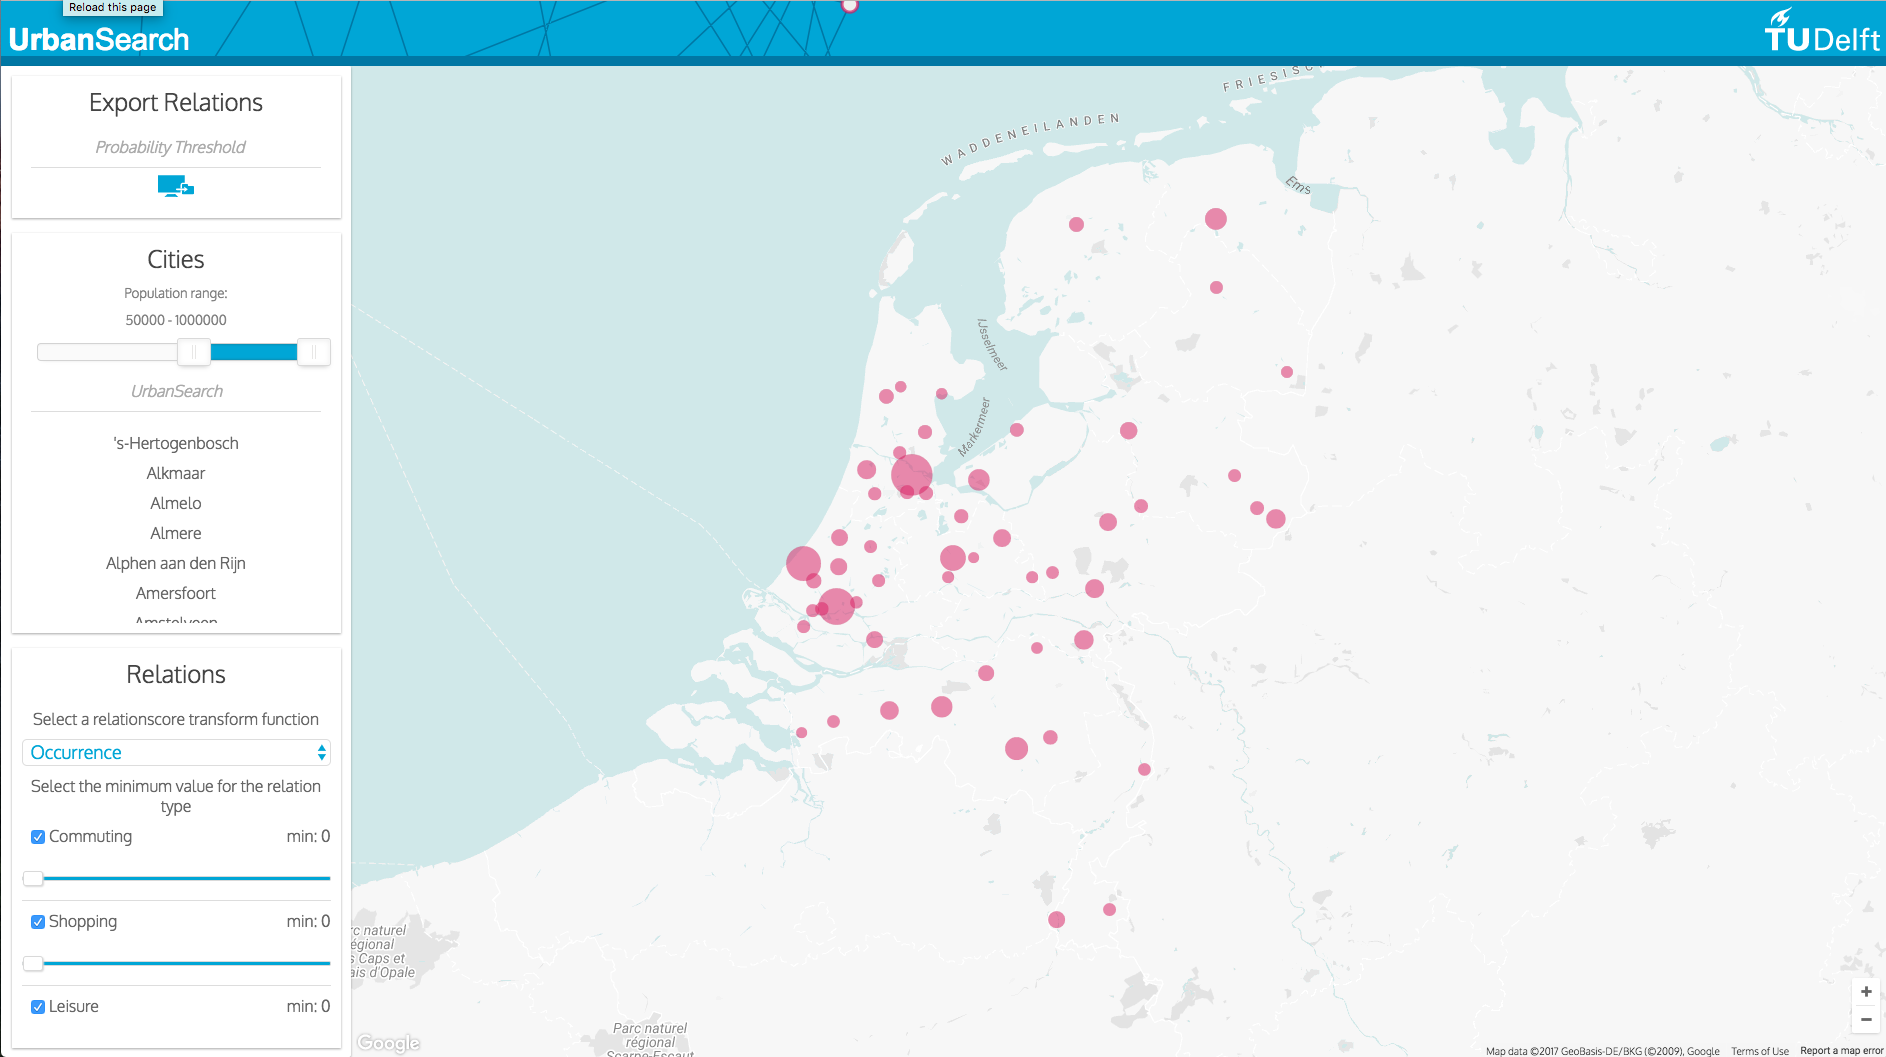
\includegraphics[scale=.5]{map}
    \caption{Map}
    \label{fig:infoflow}
\end{figure}


\begin{figure}[H]
\centering
\begin{subfigure}{.5\textwidth}
  \centering
  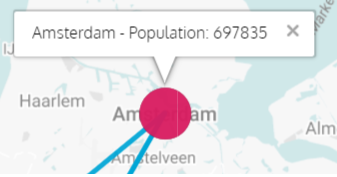
\includegraphics[width=.8\linewidth]{hover}
  \caption{Hovering over a city}
  \label{fig:sub1}
\end{subfigure}%
\begin{subfigure}{.5\textwidth}
  \centering
  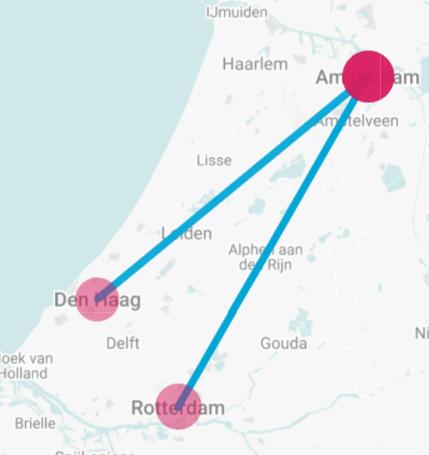
\includegraphics[width=.8\linewidth]{click}
  \caption{City showing relations}
  \label{fig:sub2}
\end{subfigure}
\label{fig:test}
\end{figure}


\subsection{Relation window}
When clicking on a relation an extra window in the menu will be opened. This contains all information about the relation between the two cities. The strength of the relations (amount of documents found for the relation between those cities) will be displayed, as well as the strength of the relations per relation type (such as commuting, shopping, leisure, ..). To check how these relationships were found the option on the lower end of this window  can be used to open up another window displaying all documents that connect those two cities.

\begin{figure}[H]
    \centering
    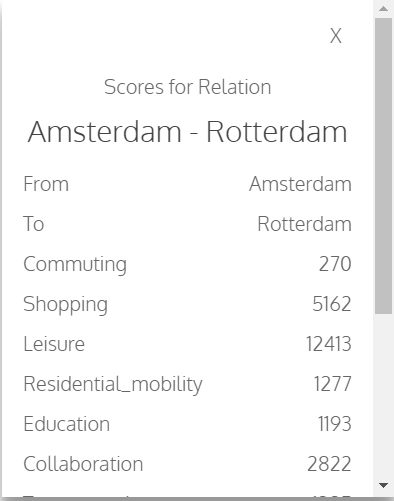
\includegraphics[scale=.7]{Score}
    \caption{Relations scores between two cities}
    \label{fig:infoflow}
\end{figure}


\subsection{Documents connecting two cities menu}
In this new window all documents will be displayed. For each document the type of relation to which the document fits and the probability this documents fits to that relation is displayed. If a document does not fit to the relation types (and is thus labelled other), it is not displayed here. The documents can be downloaded in a text file by clicking on them.

\begin{figure}[H]
    \centering
    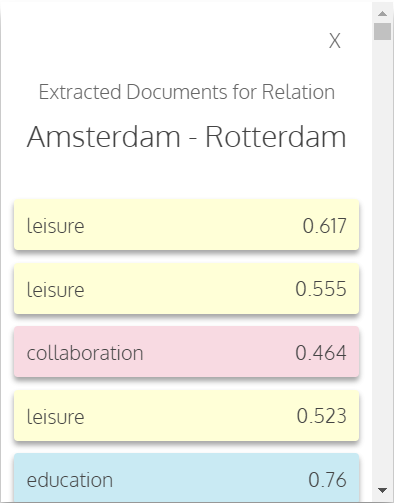
\includegraphics[scale=.7]{documents}
    \caption{Documents included in relations}
    \label{fig:infoflow}
\end{figure}

